\section{Hydrostatik}
Buch = Taschenbuch der Physik - Horst Kuchling, 22. Auflage

\subsection[Dichte]{Dichte $\bm{\rho}$}
\begin{flushright}
	$\boxed{\textbf{Buch S. 155 \& 158 }}$
\end{flushright}

\hspace*{\fill}
\begin{minipage}[c]{0.48\columnwidth}
	$$ \boxed{ \rho = \frac{m}{V} \quad \Leftrightarrow \quad m = \rho \cdot V } $$	 
\end{minipage}
\hfill
\begin{minipage}[c]{0.48\columnwidth}
	\begin{tabular}{c l c}
		$\rho$  & Dichte    & $[\rho] = \frac{\kilogram}{\meter^3}$ \\
		$m$     & Masse     & $[m] = \kilogram$                     \\
		$V$     & Volumen   & $[V] = \meter^3$
	\end{tabular}
\end{minipage}

\vspace{0.2cm}

Wie viel Masse pro $m^3$ ist.

\subsubsection{Wichtige Dichten}	

\begin{tabular}{l c l}
	$\rho_{\rm Wasser} = 1000 \, \frac{\kilogram}{\meter^3}$    & &  $\rho_{\rm Luft} = 1.2 \, \frac{\kilogram}{\meter^3}$
	
\end{tabular}


\subsection[Druck / Schubspannung]{Druck $\bm{p}$ / Schubspannung $\bm{\tau}$}

\begin{flushright}
	$\boxed{\textbf{Buch S. 153 \& 188}}$
\end{flushright}

\textbf{Druck ist eine skalare Grösse (hat keine Richtung)- Schubspannun berücksichtigt man vor allem in realen Fluiden} 

$$\boxed{ p = \frac{F_{\perp}}{A} } \qquad \qquad \boxed{ \tau = \frac{F_{\parallel}}{A} } $$

\begin{tabular}{c l c}
    $p$             & Druck                         & $[p] = \pascal = \frac{\newton}{\meter^2}$    \\
    $\tau$          & Schubspannung (Scherkraft)    & $[\tau] = \frac{\newton}{\meter^2}$                            \\
    $F_{\perp}$     & Kraft senkrecht zu $A$        & $[F_{\perp}] = \frac{kg \cdot m}{s^2} =\newton$                       \\
    $F_{\parallel}$ & Kraft parallel zu $A$         & $[F_{\parallel}] = \frac{kg \cdot m}{s^2} = \newton$                   \\
    $A$             & Fläche                        & $[A] = \meter^2$
\end{tabular}

\medskip

\textbf{In abgeschlossenen, miteinander verbundenen Systemen herrscht ein Druck-Gleichgewicht!} 

$$ \boxed{ p_1 = p_2  \quad \Leftrightarrow  \quad \frac{F_1}{A_1} = \frac{F_2}{A_2} }$$



\subsubsection{Weitere Einheiten von Druck}

\vspace{-0.2cm}
$$ \bm{1 \, \bbar = 10^5 \pascal} \qquad \text{Absolutdruck: Vergleich zu Vakuum} $$

\begin{tabular}{ll}
    $1 \, \hecto \pascal$   & $= 100 \, \pascal = 1 \, \milli \bbar $                                       \\
    $1 \, \mathrm{at}$      & $= 1 \, \mathrm{kp \cdot \centi \meter^{-2}} = 9.81 \cdot 10^4 \, \pascal$    \\
    $1 \, \mathrm{at"u}$    & $= 1 \, \mathrm{at}$ (Überdruck; Vergleich zu normalem Luftdruck)             \\
    $1 \, \mathrm{Torr}$    & $= \frac{1}{760} \, \mathrm{at}$ (1 mm-Hg-Säule)
\end{tabular}


\subsection{Boyle-Mariotte}	
\begin{flushright}
	$\boxed{\textbf{Buch S. 159}}$
\end{flushright}
\textbf{Das Gesetz von Boyle-Mariotte beschreibt die Kompressibilität von Gasen.} \\
\colorbox{violet}{ \textrightarrow\ Das Gesetz gilt nur bei konstanter Temperatur} 

$$ \boxed{ p_1 \cdot V_1 = p_2 \cdot V_2 = \, \const \quad \Leftrightarrow \quad \frac{p_1}{p_2} = \frac{\rho_1}{\rho_2} } $$ 

\renewcommand{\arraystretch}{1.3}
\begin{tabular}{c l c}
    $\rho_x$    & Gas-Dichte    & $[\rho_x] = \frac{\kilogram}{\meter^3}$   \\
    $p_x$       & Gas-Druck     & $[p_x] = \pascal $                        \\
    $V_x$       & Volumen       & $[V_x] = \meter^3$
\end{tabular}
\renewcommand{\arraystretch}{1}


\subsection{Hydrostatischer Druck (Schweredruck)}
\begin{flushright}
	$\boxed{\textbf{Buch S. 155}}$
\end{flushright}

\textbf{Gilt nur für Flüssigkeiten \newline ->im Anhang Bild zum Hydrostatischen Paradoxon} 

$$ \boxed{ p = \rho \cdot g \cdot h }$$	

\renewcommand{\arraystretch}{1.3}
\begin{tabular}{c l c}
    $\rho$  & Dichte der Flüssigkeit                                    & $[\rho] = \frac{\kilogram}{\meter^3}$ \\
    $h$     & Höhe \textbf{unter} der Flüssigkeits-Oberfläche           & $[h] = \meter$                        \\
    $g$     & Erdbeschleunigung $g = 9.81 \, \frac{\meter}{\second^2}$  & $[g] = \frac{\meter}{\second^2}$
\end{tabular}
\renewcommand{\arraystretch}{1}

\smallskip

\textbf{Der Druck ist nur von der Höhe der darüberliegenden Flüssigkeit abhängig, nicht von deren Volumen oder Gewicht.}


\subsection{Statischer Auftrieb (Fluid)}

\begin{flushright}
	$\boxed{\textbf{Buch S. 157}}$
\end{flushright}

Der Auftrieb eines Körpers entspricht dem Gewicht der von ihm verdrängten Flüssigkeit (Archimedes). 


\begin{minipage}{0.6\columnwidth}
   $$  \boxed{ F_A = F_{\rm G,Fl} = m_{\rm Fl} \cdot g} $$
   $$ \rightarrow \boxed{ F_A = \rho_{\rm Fl} \cdot V_K \cdot g } $$
\end{minipage}
\hfill
\begin{minipage}{0.28\columnwidth}
    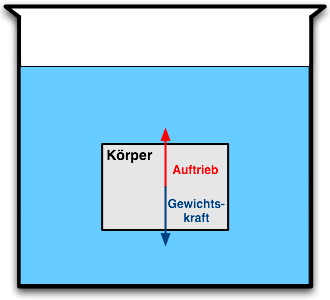
\includegraphics[width=\columnwidth]{images/auftrieb.jpg}
\end{minipage}

\smallskip

\renewcommand{\arraystretch}{1.3}
\begin{tabular}{c l c}
    $F_A$           & Auftriebskraft                                        & $[F_A] = \newton$                                 \\
    $\rho_{\rm Fl}$ & Dichte \textbf{verdrängtes Fluid}                     & $[\rho_{\rm Fl}] = \frac{\kilogram}{\meter^3}$    \\
    $V_K$           & Verdrängtes Fluid-Volumen                             & $[V_K] = \meter^3$                                \\
    $g$         & Erdbeschleunigung $g = 9.81 \, \frac{\meter}{\second^2}$  & $[g] = \frac{\meter}{\second^2}$                  \\
    $m_{\rm Fl}$    & Masse des \textbf{verdrängten Fluids}                 & $[m_{\rm Fl}] = \kilogram$                        \\
    $F_{\rm G,Fl}$  & Gewichtskraft \textbf{verdrängtes Fluid}              & $[F_{\rm G,Fl}] = \newton$
\end{tabular}
\renewcommand{\arraystretch}{1}


\subsection{Kompression - barometrische Höhenformel}

\begin{flushright}
	$\boxed{\textbf{Buch S. 157 \& 161}}$
\end{flushright}

$$ \boxed{ \text{Flüssigkeiten:} \qquad \Delta p = \frac{1}{\kappa} \cdot - \frac{\Delta V}{V} = K \cdot - \frac{\Delta V}{V} } $$  
$$ \boxed{ \text{Gase:} \qquad \Delta p = p(h) - p_0 = \frac{1}{\kappa_T} \cdot - \frac{\Delta V}{V} } $$


\begin{tabular}{c l c}
	$\Delta p$              & Druckerhöhung                     & $[\Delta p] = \pascal = \frac{\newton}{\meter^2}$     \\
	$\kappa$                & Kompressibilität (Flüssigkeit)    & $[\kappa] = \frac{1}{\pascal}$                        \\
	$K = \frac{1}{\kappa}$  & Kompressionsmodul                 & $[K] = \pascal$                                       \\
	$\kappa_T$              & Kompressibilität (Gas)            & $[\kappa_T] = \frac{1}{\pascal}$                      \\
	$- \frac{\Delta V}{V}$  & realtive Volumen-Abnahme          & $\Big[ \frac{\Delta V}{V} \Big] = 1$ 
\end{tabular}


\subsection{Oberflächenspannung}
\begin{flushright}
	$\boxed{\textbf{Buch S. 181 }}$
\end{flushright}

(Bügelmethode) \\
\begin{minipage}[c]{0.3\columnwidth}
    $$ \boxed{ \sigma = \frac{F_\sigma}{2l} = \frac{F_1-F_2}{2l} } $$ 
\end{minipage}
\hfill
\begin{minipage}[c]{0.65\columnwidth}
    \renewcommand{\arraystretch}{1.3}
    \begin{tabular}{c l c}
    $\sigma$    & Oberflächenspannung   & $[\sigma] = \frac{\newton}{\meter}$   \\
    $F$         & Kraft                 & $[F] = \newton$                       \\
    $l$         & Länge                 & $[l] = \meter$
    \end{tabular}
    \renewcommand{\arraystretch}{1}
\end{minipage}

\medskip

\textbf{Hinweis:} Die Länge $\bm{l}$ entspricht der gesamten Berührungslänge zwischen Flüssigkeit und Festkorper / Gas

\subsubsection{Druck in Flüssigkeitskugel, Gasblase}

\begin{minipage}[c]{0.3\columnwidth}
	$$ \boxed{ p = \frac{2 \cdot \sigma}{r} } $$ 
\end{minipage}
\hfill
\begin{minipage}[c]{0.66\columnwidth}
	\renewcommand{\arraystretch}{1.3}
	\begin{tabular}{c l c}
		$\sigma$    & Oberflächenspannung       & $[\sigma] = \frac{\newton}{\meter}$ \\
		$r$         & Radius der Seifenblase    & $[r] = \meter$
	\end{tabular}
	\renewcommand{\arraystretch}{1}
\end{minipage} \newline


\subsection[Kapillarität]{Kapillarität $F_{\sigma} = F_{G_{Fl}} \rightarrow \bm{h}$}
\begin{flushright}
	$\boxed{\textbf{Buch S. 183}}$
\end{flushright}

$$\boxed{  h = \frac{2 \cdot \sigma}{\rho \cdot g \cdot R} = \frac{\sigma}{\rho \cdot g \cdot d} = \frac{2 \cdot \sigma \cdot \cos(\varphi)}{\rho \cdot g \cdot r} }$$ 


\begin{tabular}{c l c}
	$\sigma$ & Totale Grenzflächenspannung            & $[\sigma] = \frac{\newton}{\meter}$   \\
	 $\rho$  & Dichte der Flüssigkeit                 & $[\rho] = \frac{\kilogram}{\meter^3}$ \\
	  $R$    & Radius der Kapillare (Krümmungsradius) & $[R] = \meter$                        \\
	  $d$    & Durchmesser der Kapillare              & $[r] = \meter$                        \\
	  $r$    & Durchmesser der Röhre                  & $[R] = \meter$ \\
	  $\varphi$ & Kontaktwinkel & $[\varphi] = x\degree$
\end{tabular}

\vspace{0.2cm}
\textbf{Hinweis:} bei $0\degree = $ Ideale Benetzung, daher fällt dann der $\bm{cos}$ weg.

\medskip

\begin{minipage}[b]{0.4\columnwidth}
    \begin{center}
        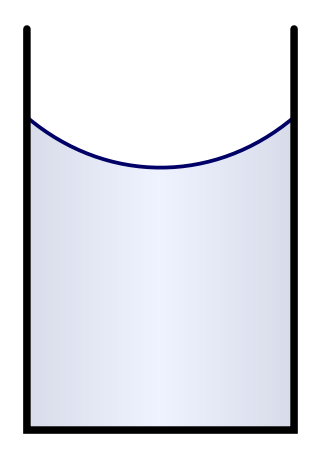
\includegraphics[width=0.25\columnwidth]{images/kapillaritaet_benetzend.png}

        benetzend $\varphi < 90^{\circ}$
    \end{center}
\end{minipage}
\hfill
\begin{minipage}[b]{0.4\columnwidth}
    \begin{center}
        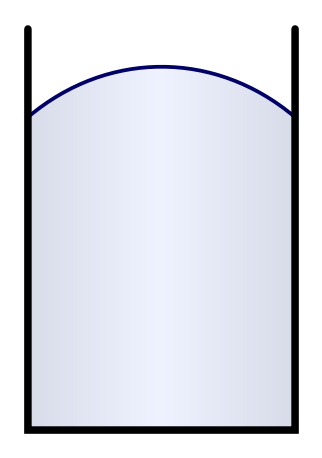
\includegraphics[width=0.25\columnwidth]{images/kapillaritaet_nicht_benetzend.png}
        
        nicht benetzend $\varphi > 90\degree$
    \end{center}
\end{minipage}

\subsubsection{Kontaktwinkel}
\hspace*{\fill}
\begin{minipage}[c]{0.3\columnwidth}
$$\boxed{\sigma_{sl} + \sigma_{lg} \cos(\varphi) = \sigma_{sg}} $$
\vspace{0.07cm}
$$
\cos \varphi = \left. \frac{\sigma_{sg} - \sigma_{sl}}{\sigma_{lg}} \right\} 
\begin{array}{l}
	\leqslant 1 \\
	\geqslant -1
\end{array}
$$ 
\end{minipage}
\hfill
\begin{minipage}[c]{0.5\columnwidth}
	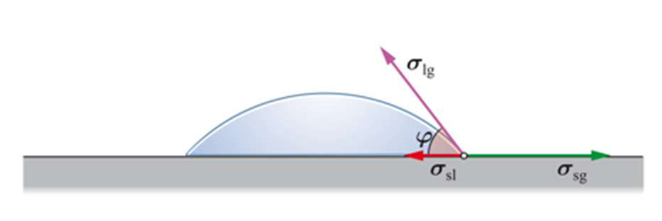
\includegraphics[scale=0.4]{images/Kontaktwinkel.png}
\end{minipage}
\hspace*{\fill}


\columnbreak